\subsection{Sprawdzenie algorytmu na innym zbiorze danych}\label{eksperyment6}
W przeprowadzonych eksperymentach osiągane wyniki nie były zadowalające. Poprawność klasyfikacji nie przekroczyła nawet $90\%$. Aby sprawdzić czy skrypt sieci neuronowej został wykonany poprawnie, wykorzystano zbiór danych $Iris$. Jest to na tyle popularny zestaw, że znalazł swoje miejsce w domyślnych zestawach danych oprogramowania Matlab R2019a. Zbiór zawiera 3 klasy po 50 rekordów, które odnoszą się do rodzaju kwiatu irysa.\\
Przeprowadzono test dla domyślnych parametrów adaptacyjnych. Zmieniana była jedynie liczba neuronów w obu warstwach w zakresie od 10 neuronów do 70 z krokiem 10.
\begin{figure}[!h]
\centering
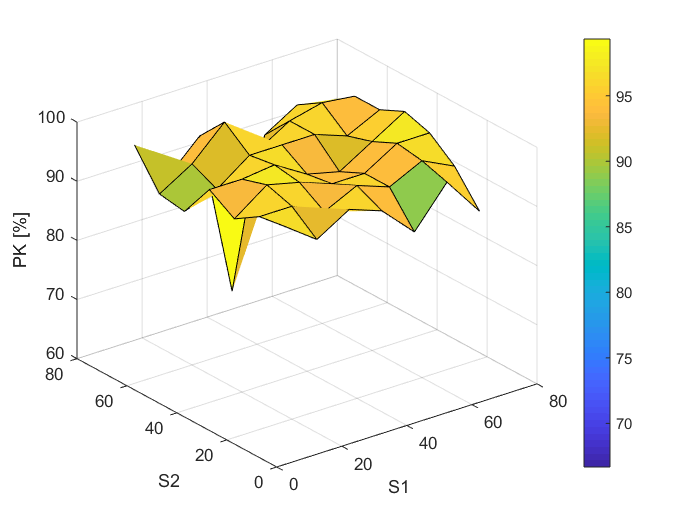
\includegraphics[width = 0.7\textwidth]{Grafika/iris_PK.png}
\caption{Wpływ liczby neuronów w warstwie pierwszej i drugiej na poprawność klasyfikacji}
\label{fig:iris_PK}
\end{figure}

Osiągnięte wyniki były zauważalnie lepsze, co potwierdza poprawność algorytmu. Dla większości konfiguracji uzyskano poprawność klasyfikacji powyżej $90\%$. Największą poprawność klasyfikacji ($99.33\%$) uzyskano dla 30 neuronów w warstwie pierwszej i 60 neuronów w warstwie drugiej.